% !TEX program = xelatex
\documentclass[journal]{IEEEtran}

\usepackage{amsmath,amssymb}
\usepackage{booktabs}
\usepackage{graphicx}
\usepackage{array}
\usepackage{multirow}
\usepackage{url}
\usepackage[colorlinks=true,allcolors=blue]{hyperref}

\newcommand{\ml}[1]{\textsc{#1}}

\begin{document}

\title{When Simulation-Based Sample Supplementation Fails in Cross-Domain Bearing
Fault Diagnosis: The Recording-Fingerprint Effect and an Evaluation Protocol
That Reveals It}

\author{%
\IEEEauthorblockN{Fangyu Zhang}
\IEEEauthorblockA{College of Mechanical and Aerospace Engineering, Jilin
University, Changchun 130025, China\\
Email: fyzhang9925@mails.jlu.edu.cn\\
ORCID: 0009-0009-7352-1484}
\and
\IEEEauthorblockN{Julong He}
\IEEEauthorblockA{National College for Excellent Engineers, University of Science
and Technology Beijing, Beijing 100083, China\\
Email: u202541560@xs.ustb.edu.cn\\
ORCID: 0009-0003-0143-7204}%
\thanks{Corresponding author: F. Zhang.}%
}

\maketitle

\begin{abstract}
Physics-based simulation, notably ``digital twin'' generators, is a
popular source of synthetic fault samples for cross-domain bearing fault
diagnosis when labeled target data are scarce. On the standard CWRU 12\,kHz
drive-end benchmark it is \emph{structurally} unable to supply
class information. Every ``fault type $\times$ load'' cell is a \emph{single
recording}, and the class-conditional magnitude spectrum is a stable property
of it: a class's spectral envelope recurs across the four loads at cosine
$0.944$, yet is not predictable from fault physics, since a source-domain
envelope transfers to the target at $0.924$ while one estimated from five
labeled \emph{target} samples reaches $0.995$. Class identity is thus a
per-bearing \emph{recording fingerprint}. A calibrated McFadden--Smith twin
produces nine classes with near-identical
spectra and, trained on twin data alone, reaches macro-F1 $0.123$ (chance
$0.10$). The standard few-shot protocol compounds this:
support and test windows share the fingerprint, so cross-recording evaluation
lowers reported macro-F1 by $0.15$--$0.19$ (up to $0.31$) and leaves
augmentation at the level of the trivial baseline. Coloring white noise with
the target envelope is the most robust augmentation for an atypical target
recording; adding a physical impulse train degrades fidelity and
accuracy. On Paderborn, where several bearings share each class, class-mean
spectra remain indistinguishable (cosine $1.000$) although classes are defined
by damage location; there same-recording optimism of $+0.386$ splits
into session ($+0.161$) and specimen ($+0.225$) terms. The advantage of
fingerprint calibration over raw physics inverts between the benchmarks.
\end{abstract}

\begin{IEEEkeywords}
bearing fault diagnosis, benchmark evaluation, cross-domain transfer, digital
twin, few-shot learning, simulation-based data augmentation, spectral
fingerprint.
\end{IEEEkeywords}

\section{Introduction}
\label{sec:intro}

Deep models for bearing fault diagnosis are notoriously fragile under domain
shift, and the scarcity of labeled data on a newly commissioned machine makes
transfer learning unavoidable. Two families of remedies dominate the
literature: (i) unsupervised domain adaptation, typically adversarial
\cite{ganin2016dann} or moment-matching \cite{sun2016coral}, and (ii) the
generation of additional labeled samples
for the target operating condition, either by physics-based simulation
\cite{ming2026physics, xiao2026sim2real, liu2024twin} or by generative models
\cite{shao2019gan}.

The simulation route is attractive because a physical model is, in principle,
transferable \cite{karniadakis2021piml, tao2019dt}: bearing characteristic
frequencies scale with shaft speed, so a
model of a spalled outer race at $1797$\,rpm can be re-instantiated at
$1730$\,rpm without any new data. Many recent papers report that augmenting
training with simulated faults improves cross-domain accuracy
\cite{liu2024twin, xu2024dt, zhang2023dt, kumar2024dt, ming2026physics,
xiao2026sim2real}.

This paper asks a prior question: \emph{what class-related information can a
physical simulator actually supply on the benchmarks we use to test it?} We
answer it for the most widely used benchmark, the CWRU 12\,kHz drive-end
dataset. There the simulator supplies essentially nothing, for a structural
reason, and the protocol used to evaluate such methods inflates the results it
reports.

\subsection{Contributions}
\begin{itemize}
\item \textbf{C1 (diagnosis).} A physically calibrated twin remains
$99.99\%$ separable from real data under a domain discriminator, and a
classifier trained only on twin data transfers to the real target domain at
macro-F1 $=0.123$, i.e.\ chance for ten classes (Section~\ref{sec:diag1}).
\item \textbf{C2 (root cause).} Class identity in CWRU is dominated by a
\emph{recording fingerprint}. Per-class spectral envelopes are stable across
loads (cosine $0.944$ averaged over all load pairs), but the source-domain
envelope predicts the target-domain envelope only to $0.924$. The twin
reproduces neither (Section~\ref{sec:diag2}).
\item \textbf{C3 (protocol).} The few-shot evaluation protocol draws support
and test windows from the same recording, so both share the fingerprint. Under
a cross-recording protocol the reported macro-F1 drops by $0.15$--$0.19$
(average over four support domains; up to $0.31$), and augmentation-based
methods become indistinguishable from training on the labeled support set alone
(Section~\ref{sec:protocol}). We recommend this control for future work.
\item \textbf{C4 (constructive).} Estimating the per-class spectral envelope
from $k$ labeled target samples is accurate ($0.995$ cosine at $k=5$), and
coloring white noise with it is the most robust augmentation when the target
recording is atypical. Adding a physical impulse train on top of it
\emph{degrades} both domain fidelity and accuracy, consistently across
settings (Sections~\ref{sec:method} and~\ref{sec:results}).
\item \textbf{C5 (side finding).} Load~3 of CWRU is an outlier operating
condition: a label-free model transfers among loads 0--2 at $0.93$--$1.00$ but
reaches only $0.71$ on load~3, and labeled support from the other loads
transfers into load~3 at $0.68$--$0.77$. Conclusions drawn from the popular
S0$\rightarrow$S3 direction alone do not generalize
(Section~\ref{sec:protocol}).
\item \textbf{C6 (cross-benchmark).} On Paderborn, where several independent
bearings share each damage class, class-mean magnitude spectra of healthy,
inner-ring and outer-ring bearings are identical (cosine $1.000$; CWRU:
$0.626$), and remain so after the dominant rig tone is filtered out (margin
$+0.003$). The CWRU class separation is therefore a property of the individual
specimens, not of the classes. Same-recording evaluation is optimistic by
$+0.386$ macro-F1 there; because each Paderborn bearing was measured $20$
times, that optimism can be split by re-evaluating on a different
\emph{recording of the same bearings}, which gives $+0.161$ for the session
and a further $+0.225$ for the change of specimen, and it survives removal of
the rig tone that holds $93\%$ of the spectral energy ($+0.321$ remains). A twin whose physics
exactly matches the class definition is still the worst augmentation tried. The
advantage of fingerprint calibration over raw physics inverts between CWRU and
Paderborn in the direction the mechanism predicts, which serves as a positive
control (Section~\ref{sec:paderborn}).
\end{itemize}

\section{Related Work}
\label{sec:related}

\paragraph{Cross-domain and few-shot bearing diagnosis}
The problem setting we study is standard: a model trained under one operating
condition must be reused under another, and labels are scarce on the target
\cite{lei2020roadmap, zhao2020benchmark}. The dominant response is unsupervised
domain adaptation, usually adversarial, which aligns source and target feature
distributions without target labels \cite{ganin2016dann, wang2018dasurvey,
zhao2021transfer}. A complementary line
attacks label scarcity directly through meta-learning and metric-based few-shot
schemes \cite{wang2020fewshot}, while the backbone architectures themselves are
now well surveyed \cite{jiao2020cnn}. Both are typically evaluated on CWRU or a
handful of sibling benchmarks, and both depend on the support set being
representative of the target test distribution. We show that under the usual
window-level split this assumption is violated in a specific and quantifiable
way.

\paragraph{Simulation and digital-twin sample supplementation}
Because a physical model transfers by construction, generating labeled fault
samples by simulation is attractive precisely when target labels are missing.
Recent work builds bearing dynamics models and uses the resulting \emph{twin
data} as a labeled source: partial domain adaptation driven by a digital twin
\cite{zhang2023dt}, discriminative graph learning that transfers knowledge from
simulated to real signals \cite{xu2024dt}, multimode collaborative transfer
learning on twin samples \cite{liu2024twin}, and digital-twin-assisted domain
adversarial frameworks for machinery such as centrifugal pumps
\cite{kumar2024dt}. A recurring theme in this literature is the
simulation-to-reality gap, and much of the machinery --- physics-enhanced
translation between simulated and measured signals \cite{ming2026physics},
generative alignment of the two distributions \cite{xiao2026sim2real} --- exists
to close it. The same gap motivates domain randomization in robotics
\cite{tobin2017domain}, where the simulator is deliberately not made faithful
and the burden shifts entirely onto the augmentation distribution.

Our contribution is orthogonal to closing that gap. We ask what
class-discriminative information the simulated data can carry in the first
place, given the structure of the benchmark, and we answer it with a negative
result that no amount of gap-closing can repair: on CWRU the class-conditional
spectrum is a property of the individual recording rather than of the fault, so
a simulator with perfect fidelity to the physics still cannot supply the
contrast that separates the classes.

\paragraph{Surrogate data}
Our phase-randomization control follows the standard surrogate-data procedure
for testing whether a statistic depends on structure beyond the power spectrum
\cite{theiler1992surrogate, schreiber2000surrogate}. We use it in the reverse
direction from the usual
application: rather than asking whether a signal is nonlinear, we use
phase-randomized surrogates as a deliberately \emph{structure-free} augmentation
baseline, to separate the contribution of the spectral envelope from that of any
temporal structure.

\section{Data, Taxonomy and Protocol}
\label{sec:setup}

\subsection{CWRU and the ten-class taxonomy}
We use the CWRU 12\,kHz drive-end recordings \cite{smith2015cwru}. The
conventional four-class
taxonomy (normal, ball, inner race, outer race) is saturated on cross-load
transfer --- a source-only model reaches $100\%$ accuracy in all twelve
transfer directions --- so we adopt a ten-class taxonomy:
$\{\textsc{Normal}\} \cup \{B,IR,OR\} \times \{0.007'', 0.014'', 0.021''\}$,
using the official files for the four loads $\{0,1,2,3\}$
($1730$--$1797$\,rpm). Windows of $1024$ samples with stride $512$ are
$z$-scored individually.\footnote{Every spectral scalar reported in this paper
is reproduced from the raw data by one script released with the code
(\texttt{tools/probe\_spectral\_numbers.py}), and every table entry by
\texttt{tools/verify\_paper\_numbers.py}.}

\subsection{The few-shot split}
For a target load, each class is split in time order: the last $40\%$ of
windows form the held-out test set; from the first $60\%$, $k$ windows per
class are drawn (with the seed) as the labeled \emph{support} set, and the rest
form an unlabeled \emph{pool}. Crucially, the support and test windows come
from the \emph{same recording}. Section~\ref{sec:protocol} shows how much of
the reported score that choice accounts for.

\subsection{Classifier and training}
\label{sec:classifier}
Every configuration is trained with the same model, so that each comparison
isolates the training set rather than the architecture. The input is the raw
time-domain window, $z$-scored sample-wise, and no spectral transform is applied
before the classifier: the spectral statistics of
Sections~\ref{sec:diag1} and~\ref{sec:diag2} are diagnostics on the data, not
features of the model. The backbone is a one-dimensional residual network with a
$7$-tap convolution (stride $2$, $32$ channels), batch normalisation and ReLU,
three residual blocks of two $3$-tap convolutions each ($32$, $64$ and $128$
channels, stride $2$ from the second block), global average pooling, and a
linear projection to $64$ features. One linear layer maps those features to
class scores, and the domain discriminator used by the adversarial methods is a
two-hidden-layer MLP of width $64$ on the same features. The backbone has
$118\,368$ parameters and the model $127\,403$ including the discriminator.
Training minimises cross-entropy, plus a binary domain loss where a
discriminator is used, with Adam at a learning rate of $10^{-3}$, batch size
$64$ and $60$ epochs, $200$ for the Paderborn comparisons of
Section~\ref{sec:paderborn}; synthetic sets are generated with $400$ windows per
class. One seed controls the few-shot draw, the synthetic sample generation and
the weight initialisation jointly.

\section{Diagnosis I: What the Twin Supplies}
\label{sec:diag1}

\subsection{The generator}
We implement a McFadden--Smith style impulse-response twin
\cite{randall2011rolling} with SKF 6205-2RS geometry, whose
ball-pass frequencies are computed from the shaft speed. The generator is
calibrated against real CWRU spectra: the resonance range, the resonance
bandwidth per defect size, the background-noise colouring, and the
impulse-to-harmonic power ratio were all fitted so that synthetic
band-energy shares match measured ones. In particular the synthetic peak
envelope spectrum lands on the correct BPFO, so the twin reproduces the fault
kinematics that the benchmark labels describe.

\subsection{Twin data are a different domain, and carry no class information}
Training only on twin data and testing on the real target load
(Table~\ref{tab:synth}) gives macro-F1 $=0.123 \pm 0.030$ against a chance
level of $0.10$. A linear domain discriminator on backbone features separates
twin from real with accuracy $0.9999$. The same table shows the ordering that
the rest of the paper is about: the target-calibrated envelope reaches $0.910$,
and every attempt to put physical structure back on top of it \emph{lowers}
the score.

\begin{table}[t]
\centering
\caption{Training only on a synthetic source, testing on the real target load
(load~3, ten classes). Each entry is $20$ runs --- ten seeds, the whole
configuration repeated twice --- and the $\pm$ is the standard deviation over
those $20$ runs. ``Disc.''\ is a domain discriminator
trained on backbone features to separate the synthetic source from real target
data ($0.5$ = indistinguishable). The two
repetitions of the target-fingerprint row differ by $0.033$ in the mean of ten
seeds, and a single ten-seed draw would understate that row's spread by a
factor of two.}
\label{tab:synth}
\small
\resizebox{\columnwidth}{!}{%
\begin{tabular}{lcc}
\toprule
Synthetic source & macro-F1 & Disc. \\
\midrule
Physics twin (source speed)                & $0.123 \pm 0.030$ & $0.9999$ \\
Source fingerprint $+$ white noise         & $0.587 \pm 0.045$ & $0.9972$ \\
Source fingerprint $+$ impulse train       & $0.491 \pm 0.041$ & $0.9994$ \\
Target fingerprint $+$ impulse train       & $0.651 \pm 0.056$ & $0.9786$ \\
Target fingerprint $+$ impulse (comb-free) & $0.524 \pm 0.061$ & $0.9999$ \\
\textbf{Target fingerprint $+$ white noise}& $\mathbf{0.910 \pm 0.077}$ & $\mathbf{0.9337}$ \\
\bottomrule
\end{tabular}
}
\end{table}

\section{Diagnosis II: the Recording Fingerprint}
\label{sec:diag2}

\subsection{Class differences are stable across loads}
Taking the smoothed magnitude envelope $A_c(f)$ as each class's spectral
signature (Section~\ref{sec:method}), the signature of load~0 correlates with
those of loads 1--3 at cosine $0.954$, $0.939$ and $0.924$ respectively (mean
$0.939$); averaged over all six load pairs the value is $0.944$. Class
differences therefore survive a change of load and are a stable property of the
\emph{recording}, which is why real-data methods work well here.
Table~\ref{tab:bench} reports a separate, unsmoothed statistic
(Section~\ref{sec:paderborn}), which yields systematically lower cosines.

\subsection{But they are not predictable from fault physics}
The nine synthetic fault classes have near-identical mean spectra
(Fig.~\ref{fig:spectra}(b)): all occupy
$48$--$64\%$ (mean $55\%$) of their energy in the $2800$--$3300$\,Hz band,
whereas the nine real classes at load~0 spread from $9\%$ (OR014) to $67\%$
(IR021), mean $32\%$. Table
\ref{tab:classsep} quantifies this with the mean pairwise cosine distance
between class-mean spectra: real data $0.374$, twin $0.167$.

\begin{table}[t]
\centering
\caption{Mean pairwise cosine distance between class-mean magnitude spectra
(higher = classes better separated). Target load~3.}
\label{tab:classsep}
\small
\resizebox{\columnwidth}{!}{%
\begin{tabular}{lc}
\toprule
Source & Mean inter-class distance \\
\midrule
Real target (load 3)                    & $0.374$ \\
Real source (load 0)                    & $0.374$ \\
Physics twin                            & $0.167$ \\
Target fingerprint $+$ white noise      & $0.315$ \\
Target fingerprint $+$ impulse train    & $0.346$ \\
Target fingerprint (comb-free) $+$ imp. & $0.319$ \\
\bottomrule
\end{tabular}
}
\end{table}

Table~\ref{tab:classsep} also exposes a subtlety that we return to in
Section~\ref{sec:results}: the physics impulse train \emph{increases}
inter-class distance relative to the fingerprint-only condition, yet it
transfers worse. The physical structure does not destroy class information; it
pushes the sample distribution away from the real one.

\subsection{Why physics cannot close the gap}
Each CWRU fault file was recorded with a \emph{different} damaged bearing, and
the same bearing was re-used across loads for a given file. ``What this class
looks like'' is therefore a property of that particular bearing and recording
session. A simulator cannot know which bearing a target recording used. The
fingerprint is estimable from target labels (Section~\ref{sec:method}) but not
derivable from fault mechanics. In the terminology of the shortcut-learning
literature \cite{geirhos2020shortcut}, the classifier learns the recording as
the shortcut to the label; on this benchmark the shortcut is not merely easier
than the intended solution but the only signal present.

\section{Evaluation Protocol: Same-Recording Leakage}
\label{sec:protocol}

The support and test windows of the standard few-shot split come from one
recording, so they share the fingerprint. This is a leakage of the kind that
has been catalogued as a general threat to machine-learning-based science
\cite{kapoor2023leakage}: the split is drawn at the window level while the
statistical unit that carries the label is the recording, so the test set is
not independent of the training set in the sense that matters. To quantify the
resulting optimism we
evaluate every configuration twice: on the held-out windows of the
\emph{same} load, and on the \emph{other} three loads, which are different
recordings. Table~\ref{tab:leak} reports the result for $k=5$.

\begin{table*}[t]
\centering
\caption{Same-recording versus cross-recording evaluation ($k=5$, macro-F1).
Each cell is $6$ runs --- three seeds, the whole configuration repeated twice.
Each block trains on the labeled support of one load and evaluates
on its own held-out windows (\emph{same}) and on the other three loads
(\emph{cross}). ``Surrogate''\ = Fourier phase randomization of each support
sample; ``true aug''\ = $400$ real labeled samples per class drawn from the
unlabeled pool.}
\label{tab:leak}
\small
\begin{tabular}{llcccc}
\toprule
Support load & Training configuration & Same & Cross mean & Cross (to load 3) & Optimism \\
\midrule
\multirow{4}{*}{load 0}
 & support only            & $0.987$ & $0.868$ & $0.696$ & $+0.119$ \\
 & $+$ fingerprint aug.    & $0.985$ & $0.837$ & $0.709$ & $+0.148$ \\
 & $+$ phase surrogate     & $0.989$ & $0.826$ & $0.737$ & $+0.163$ \\
 & $+$ true samples        & $1.000$ & $0.864$ & $0.695$ & $+0.135$ \\
\midrule
\multirow{4}{*}{load 1}
 & support only            & $0.988$ & $0.871$ & $0.684$ & $+0.117$ \\
 & $+$ fingerprint aug.    & $0.988$ & $0.837$ & $0.691$ & $+0.151$ \\
 & $+$ phase surrogate     & $0.992$ & $0.811$ & $0.661$ & $+0.181$ \\
 & $+$ true samples        & $1.000$ & $0.894$ & $0.714$ & $+0.106$ \\
\midrule
\multirow{4}{*}{load 2}
 & support only            & $0.999$ & $0.871$ & $0.767$ & $+0.127$ \\
 & $+$ fingerprint aug.    & $0.946$ & $0.847$ & $0.733$ & $+0.099$ \\
 & $+$ phase surrogate     & $0.798$ & $0.684$ & $0.596$ & $+0.114$ \\
 & $+$ true samples        & $1.000$ & $0.929$ & $0.881$ & $+0.071$ \\
\midrule
\multirow{4}{*}{load 3}
 & support only            & $0.998$ & $0.725$ & --- & $+0.273$ \\
 & \textbf{fingerprint aug.}& $0.995$ & $\mathbf{0.809}$ & --- & $+0.186$ \\
 & $+$ phase surrogate     & $0.997$ & $0.686$ & --- & $+0.311$ \\
 & $+$ true samples        & $1.000$ & $0.688$ & --- & $+0.312$ \\
\midrule
\multicolumn{2}{l}{Mean over the four support loads} & & & & \\
\multicolumn{2}{l}{\quad support only}      & $0.993$ & $0.834$ & & $+0.159$ \\
\multicolumn{2}{l}{\quad fingerprint aug.}  & $0.979$ & $0.832$ & & $+0.146$ \\
\multicolumn{2}{l}{\quad phase surrogate}   & $0.944$ & $0.752$ & & $+0.192$ \\
\multicolumn{2}{l}{\quad true samples}      & $1.000$ & $0.844$ & & $+0.156$ \\
\bottomrule
\end{tabular}
\end{table*}

Four conclusions follow.

\paragraph{Same-recording evaluation is optimistic by $0.15$--$0.19$}
Support-only training scores $0.987$--$0.999$ on its own held-out windows but
only $0.725$--$0.871$ on other recordings (Fig.~\ref{fig:leak}). A few-shot
result on this benchmark that uses the standard split contains this optimism
unless a cross-recording control is reported alongside it.

\paragraph{No augmentation reliably beats the labeled support set}
Averaged over the four support loads, cross-recording macro-F1 is $0.834$ for
support only, $0.832$ for fingerprint augmentation, $0.844$ for adding $400$
real labeled samples per class, and $0.752$ for phase surrogates. The three
former are within noise of each other. In particular, adding large amounts of
\emph{real} data from the same operating condition does not improve
cross-recording generalization: the bottleneck is the operating condition, not
the sample count.

\paragraph{Fingerprint augmentation is a regularizer}
Its advantage appears only when the support recording is atypical. With
load~3 as the support load it reaches $0.809$ against $0.725$ for support only;
with loads 0--2 as the support load it is worse by $0.02$--$0.03$ ($0.837$
against $0.868$ on load~0). The mechanism is
that averaging the $k$ support spectra into a class-level model suppresses
recording-specific idiosyncrasies.

\paragraph{Load 3 is an outlier condition}
A purely source-trained model, using no target labels at all, transfers among
loads 0--2 at $0.93$--$1.00$ but reaches only $0.71$ when load~3 is the test
recording; conversely, labeled support from loads 0--2 transfers into load~3 at
only $0.68$--$0.77$. The widely used S0$\rightarrow$S3 direction is hard mainly
because load~3 is peculiar; results reported on that direction alone should not
be generalized.

\begin{figure*}[t]
\centering
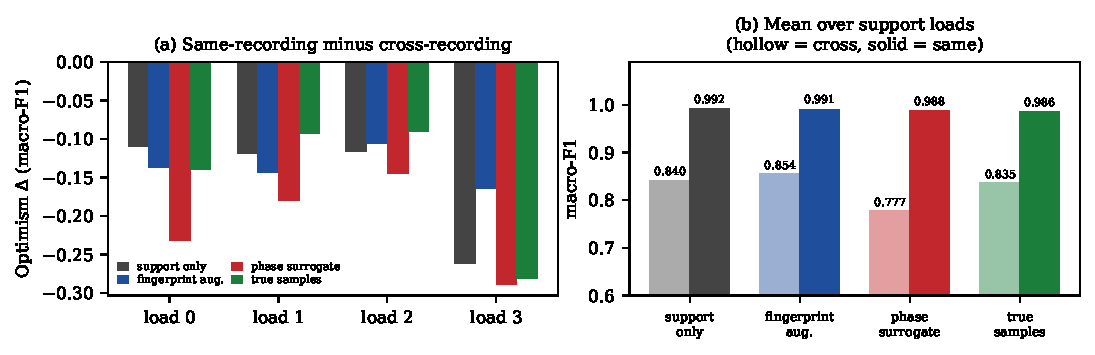
\includegraphics[width=0.98\textwidth]{figs/fig_leakage.pdf}
\caption{Same-recording versus cross-recording evaluation ($k=5$, three
seeds, two repetitions). (a)~The optimism $\Delta$ of each training configuration, per support
load: every bar is positive, i.e.\ every configuration looks better on its own
held-out windows than on other recordings, and the effect is largest exactly
where load~3 is involved --- the condition used by the most widely reported
transfer direction.
(b)~Averaged over the four support loads. Hollow bars are cross-recording,
solid bars same-recording. No augmentation reliably beats training on the
labeled support set once the evaluation is cross-recording, and adding $400$
\emph{real} labeled samples per class ($0.844$) is within noise of the trivial
baseline ($0.834$).}
\label{fig:leak}
\end{figure*}

\section{Cross-Benchmark Control: Paderborn}
\label{sec:paderborn}

CWRU cannot falsify the fingerprint explanation, because it does not contain the
control that would do so: every class has exactly \emph{one} specimen. We
therefore repeat the essential measurements on the Paderborn (KAt) dataset
\cite{lessmeier2016paderborn}, in which several independent bearings share each
damage class, measured under four operating conditions at 64\,kHz.

We use 21 bearings: 6 healthy (K001--K006), 9 artificially damaged (KA series)
and 6 damaged by accelerated lifetime tests (KI series). Classes are defined by
\emph{damage location}, read from the damage profile that ships with each
bearing (outer ring OR, inner ring IR, healthy) --- i.e.\ exactly the kinematic
distinction that a fault model can express. Windows are 4096 samples (64\,ms).
At 64\,kHz a 1024-sample window spans only 16\,ms --- barely more than one BPFO
period at 1500\,rpm ($76$\,Hz, $13$\,ms), so a window rarely holds more than one
impact --- and with 1024-sample windows all bearings produce indistinguishable
spectra, whereas the 4096-sample window holds about five periods.

In the subset we downloaded, every KA bearing is outer-ring and every KI
bearing is inner-ring, so damage location and damage origin (artificial versus
run-to-failure) are confounded. The finding below is an \emph{absence} of
class-conditional spectral structure and is unaffected, but the data cannot
support a separate statement about outer versus inner race.

\subsection{Class-conditional spectra are a rig property, not a class property}

\begin{figure*}[t]
\centering
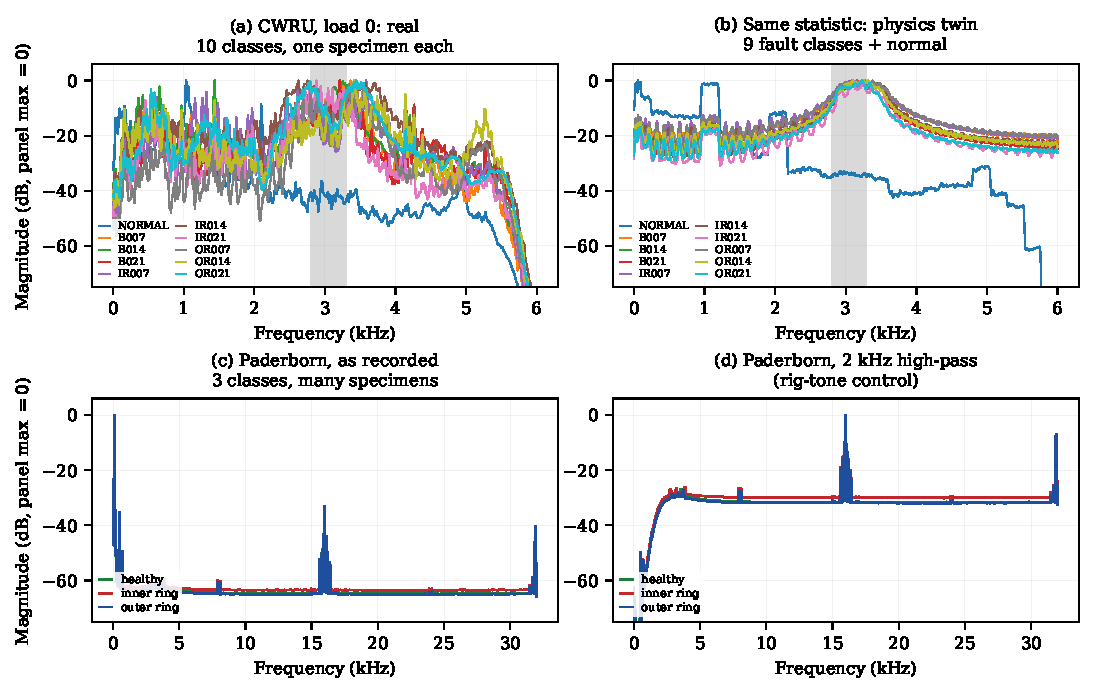
\includegraphics[width=0.98\textwidth]{figs/fig_spectra.pdf}
\caption{Class-mean magnitude spectra under the identical, unsmoothed
statistic of Table~\ref{tab:bench}. Each panel is normalized to its own maximum
(0\,dB); all four share the same $-75$\,dB floor, the same linear frequency
axis and the same per-class colours, and the shaded span marks the
$2800$--$3300$\,Hz band whose energy fraction is quoted in
Section~\ref{sec:diag2}. (a)~CWRU, ten classes, one physical specimen each:
visibly separated. (b)~The physics twin, same statistic: the nine fault classes collapse into one
band. Their median pairwise separation is $2.5$\,dB (minimum $0.9$\,dB), against
$6.7$\,dB (minimum $3.7$\,dB) for the nine real classes, and across frequency
the nine twin curves span a median of $6.5$\,dB against $18.8$\,dB. This is the
whole negative result in one panel --- the simulator produces nine faults whose
mean spectra are interchangeable, so no classifier trained on them can carry
the contrast that separates the real classes. (c)~Paderborn as recorded: the
$100$\,Hz rig line of Section~\ref{sec:paderborn} lands in the $93.75$\,Hz bin
(with leakage into its neighbour at $109$\,Hz) and carries essentially all the
energy, and the three damage
classes are indistinguishable because everything else lies $60$\,dB below it.
(d)~The same recordings after a $2$\,kHz high-pass removes that line, so the
comparison no longer rests on it. The 16\,kHz rig resonance now dominates, yet
the three class means still track each other to within a few dB across the whole
band: the absence of class structure survives removal of the tone. Compare (d)
with (a), where the same statistic separates
the real classes by $10$--$30$\,dB.}
\label{fig:spectra}
\end{figure*}

Table~\ref{tab:bench} compares the two benchmarks with one identical statistic:
the cosine similarity between class-mean magnitude spectra, shown directly in
Fig.~\ref{fig:spectra}.

\begin{table}[t]
\centering
\caption{Class-mean magnitude spectra, identical statistic on both benchmarks:
the \emph{unsmoothed} mean magnitude spectrum of each class, so the two
benchmarks are directly comparable. It is distinct from the smoothed envelope
$A_c(f)$ of Section~\ref{sec:method} used elsewhere, which yields higher
cosines.
``Within'' = different specimens, same class; ``between'' = different
specimens, different class. CWRU has one specimen per class, so only the
between-class numbers exist there; its ``same class across loads'' row is the
closest analogue of a within-class measurement. The last two rows remove the
rig tone of Section~\ref{sec:paderborn} by high-pass filtering at 2\,kHz, the
control for a dominant rig line.}
\label{tab:bench}
\small
\begin{tabular}{llcc}
\toprule
Benchmark & Quantity & Cosine & Margin \\
\midrule
\multicolumn{4}{l}{\emph{CWRU (one specimen per class)}} \\
 & between class, load 0   & $0.626$ & --- \\
 & between class, load 3   & $0.626$ & --- \\
 & same class, load 0 vs 1 & $0.870$ & --- \\
\midrule
\multicolumn{4}{l}{\emph{Paderborn ($21$ specimens)}} \\
 & within class            & $1.000$ & \\
 & between class           & $1.000$ & $+0.000$ \\
\midrule
\multicolumn{4}{l}{\emph{Paderborn, high-pass $2$\,kHz}} \\
 & within class            & $0.992$ & \\
 & between class           & $0.989$ & $+0.003$ \\
\bottomrule
\end{tabular}
\end{table}

On CWRU the ten classes are strongly separated in the magnitude spectrum
(cosine $0.626$). On Paderborn, where a class contains several independently
manufactured bearings, averaging over specimens leaves \emph{no} separation at
all: within-class and between-class cosines are both $1.000$ to three decimals.
The spectra are dominated by a rig tone: at 1500\,rpm the largest spectral line
is at $100$\,Hz --- exactly four times the shaft rate --- in \emph{every one} of
the 21 bearings (measured on the full records it falls in $99.6$--$100.1$\,Hz
for all of them), healthy, outer-ring and inner-ring alike. In a Hann-windowed
$4096$-point spectrum that line lands in the bin at $93.75$\,Hz and
\emph{that single bin} carries $54\%$ of the total spectral energy
($53.97$--$54.31\%$ across the 21 bearings); the
line together with two neighbouring bins on each side carries
$99.5$--$99.8\%$.

Because that single line holds almost all the energy, the coincidence of class
means could in principle be an artefact of it. After high-pass filtering at
2\,kHz the within-class cosine falls to $0.992$ and the between-class cosine to
$0.989$; the margin moves from $0.000$ to $+0.003$. Removing the rig tone does
not reveal a hidden class signature --- there is none in the magnitude
spectrum --- the opposite of what happens on CWRU, where the between-class
cosine stays at $0.62$--$0.63$ in every load. Filtering before \emph{training}
rather than before the statistic gives the same answer;
Section~\ref{sec:pb_filter} reports that control.

The two facts together identify the mechanism. The class separation that makes
CWRU look easy is not a property of the fault classes; it is a property of the
individual specimens and recordings that happen to carry the class labels. Where
several specimens share a label, the separation disappears.

\subsection{Same-recording leakage reproduces on a second benchmark}

A second benchmark tests whether the optimism of
Section~\ref{sec:protocol} is specific to CWRU. We train one model per seed on
five bearings per class and evaluate it twice: on held-out windows drawn from the \emph{same} bearings
($30\%$ of the training recordings), and on one bearing per class that the model
has never seen. Both test sets are class-balanced and the metric is macro-F1.
They are the two endpoints that
Table~\ref{tab:pb_levels} separates, from that same run.

\begin{table}[t]
\centering
\caption{Same-recording versus bearing-disjoint evaluation on Paderborn
(condition N15\_M07\_F10, three classes, 5 training bearings per class, 200
epochs, ten seeds, macro-F1). The training set is files 1--4 of the training
bearings; the same-recording test set is its held-out $30\%$ of windows. All
ten runs are included, including the one that did not converge (see the text
below).}
\label{tab:pb_leak}
\small
\resizebox{\columnwidth}{!}{%
\begin{tabular}{lccc}
\toprule
 & Same recording & Bearing-disjoint & Optimism \\
\midrule
Mean over 10 seeds & $0.891$ & $0.505$ & $+0.386$ \\
Std. deviation     & $0.120$ & $0.161$ & \\
\midrule
\multicolumn{4}{l}{\emph{CWRU, for comparison} (mean over four support loads)} \\
Support only      & $0.993$ & $0.834$ & $+0.159$ \\
\bottomrule
\end{tabular}
}
\end{table}

The optimism is $+0.386$, well above the CWRU average and above CWRU's worst
case. It is a consequence of drawing support and test windows from one
recording, and it reproduces wherever a benchmark is organized as a small number
of long recordings. Under a bearing-disjoint protocol the features do retain
\emph{some} transferable signal ($0.505$ against $0.333$ chance), but of the
$0.558$ by which the same-recording score exceeds chance, $0.386$ is optimism.

The spread is larger here than on CWRU, and one of the ten runs deserves a
comment. Seed~6 failed to converge: its macro-F1 on the \emph{training} set is
$0.60$ where the other nine reach $0.98$--$1.00$, and all three of its test
scores are correspondingly low. Re-running the identical configuration
converged ($1.00$ on the training set, $L1 = 0.927$), so this is a transient
optimization failure rather than a property of the split. We report it rather than
replace it: the contrast is measured \emph{within} a run, and its optimism,
$+0.12$, is the smallest of the ten (the other nine span $+0.13$ to $+0.66$).
Discarding it would have raised the same-recording mean from $0.891$ to
$0.931$.

\subsection{The optimism decomposes into a session term and a specimen term}

The two endpoints above leave the decisive question open: between them,
\emph{two} factors change at once. The bearing-disjoint test set is a different recording session \emph{and}
a different physical bearing. CWRU cannot separate them, because each class is a
single specimen. Paderborn can, because each of the numbered bearings was
measured $20$ times under the same condition: a model can be trained on files 1--4 of a
set of bearings and tested on files 5--8 of exactly those same bearings --- a
different recording session of the same specimen. The three test sets are drawn
as a ladder in Fig.~\ref{fig:pb_levels}(a), where the drop between consecutive
points is exactly one of the two terms computed below.

\begin{table}[t]
\centering
\caption{Decomposing the optimism, and the same decomposition with the rig tone
removed. One training set (files 1--4 of five bearings per class, first $70\%$
of windows) is evaluated on three test sets that differ by exactly one factor
each: L2 moves only the recording session, L3 moves the specimen as well. Same
condition, epochs and seeds as Table~\ref{tab:pb_leak}; the \emph{no filter}
column is that table's two endpoints. In the last two columns every window is
masked in the frequency domain and renormalised before training, and the whole
procedure is repeated from scratch: the notch removes $100$\,Hz and its first
twenty harmonics with $\pm2$ bins each, and the high-pass is the $2$\,kHz
control of Table~\ref{tab:bench}.}
\label{tab:pb_levels}
\small
\resizebox{\columnwidth}{!}{%
\begin{tabular}{lccc}
\toprule
 & No filter & Notch & High-pass \\
\midrule
Spectral energy removed        & ---      & $93.3\%$ & $99.7\%$ \\
L1 same file, held-out windows & $0.891$  & $0.899$  & $0.908$ \\
L2 files 5--8, same bearings   & $0.730$  & $0.772$  & $0.776$ \\
L3 held-out bearings           & $0.505$  & $0.577$  & $0.550$ \\
\midrule
Session term (L1$-$L2)         & $+0.161$ & $+0.127$ & $+0.132$ \\
Specimen term (L2$-$L3)        & $+0.225$ & $+0.195$ & $+0.226$ \\
Total optimism (L1$-$L3)       & $+0.386$ & $+0.321$ & $+0.358$ \\
\bottomrule
\end{tabular}
}
\end{table}

Both terms are positive, and the specimen term is the larger. Simply
re-measuring the \emph{same} bearings costs $+0.161$ macro-F1: that much
of the optimism is pure session leakage, with the specimen held fixed. Changing
the specimen on top of that costs a further $+0.225$. The two explanations that
the CWRU protocol cannot distinguish --- ``the model keys on the recording'' and
``the model keys on the individual bearing'' --- are therefore both real, with
the specimen carrying the larger share.

Two qualifications belong here. First, the specimen term is far more variable
than the session term: dropping it has a standard deviation of $0.209$ against
$0.046$ for the session drop, and one of ten seeds (seed~3, $L3 = 0.77$) even
reverses the sign. Which bearing is held out matters more than which session it
was measured in, as expected if the specimen term is carried by that
bearing's individual spectral signature. The ten splits between them draw on
$15$ of the $21$ bearings (five of the six healthy, four of the six inner-ring
and six of the nine outer-ring), so what varies across seeds is a property of
specimens in general rather than one unlucky draw.

Second, $L3 = 0.505$ is well above
chance, so cross-specimen transfer is not zero: part of the fault physics does
survive the change of specimen. Neither term rests on a handful of runs: over
the ten seeds the session term is positive in all ten and the specimen term in
nine, a two-sided sign test giving $p = 0.002$ and $p = 0.021$ without any
normality assumption, and the $95\%$ confidence intervals for the two means are
$+0.128$ to $+0.193$ and $+0.076$ to $+0.374$. Nor is the decomposition a property of this one network: a ResNet
with a quarter of the parameters ($30\,099$ against $118\,368$) and the same
recipe gives $L1 = 0.883$, $L2 = 0.727$, $L3 = 0.537$ --- session $+0.156$,
specimen $+0.189$, the same ordering and the same total to within $0.04$ (its
ten runs reach a training macro-F1 of $0.98$ on average, two of them $0.88$).

\subsection{The decomposition is not carried by the rig tone}
\label{sec:pb_filter}

The $100$\,Hz line of Section~\ref{sec:diag2} belongs to the test rig rather
than to any bearing, so it cannot encode a specimen's identity. Because it
dominates the spectrum, however, it could carry much of the class structure on
its own, and the decomposition might then measure little more than the recovery
of that one line. To test this we remove the line before training and repeat the
whole decomposition with the same splits, seeds and schedule. Two filters are used: a
notch at $100$\,Hz and its first twenty harmonics, $\pm2$ bins each, which
discards $93.3\%$ of the spectral energy of the untapered window, and the
$2$\,kHz high-pass of Table~\ref{tab:bench}, which discards $99.7\%$.

Both filters leave the conclusion of the section standing
(Table~\ref{tab:pb_levels}). Same-recording evaluation moves little --- L1 is
$0.899$ and $0.908$ against $0.891$ unfiltered --- although more than nine
tenths of the energy is gone. Total optimism is $+0.321$ and $+0.358$ against
$+0.386$. The session term is the one that moves consistently: it falls to
$+0.127$ and $+0.132$ from $+0.161$, a paired reduction of $0.034 \pm 0.012$
and $0.028 \pm 0.011$ standard error, and it is lower in nine of the ten seeds
under each filter --- the exception is the run of the previous subsection that
did not converge. The specimen term moves by $-0.030 \pm 0.018$ under the notch
and by $+0.001 \pm 0.023$ under the high-pass, i.e.\ in no direction that the
two filters agree on, so we read it as unchanged. Roughly a fifth of the session
leakage is therefore carried by the dominant line; the rest of it, and the
whole of the specimen term, lie in the remainder of the spectrum --- the bearing
resonances and their sidebands, which is where the fault signature itself is.

Discarding more than $99\%$ of the signal energy still leaves a same-recording
optimism of $0.32$--$0.36$: the effect is not an artefact of one conspicuous
spectral line, and notch-filtering the input does not remove it.
Fig.~\ref{fig:pb_levels} draws the same numbers: in (a) the three ladders are
nearly parallel, and in (b) the session bars fall under either filter while the
specimen bars do not.

\begin{figure*}[t]
\centering
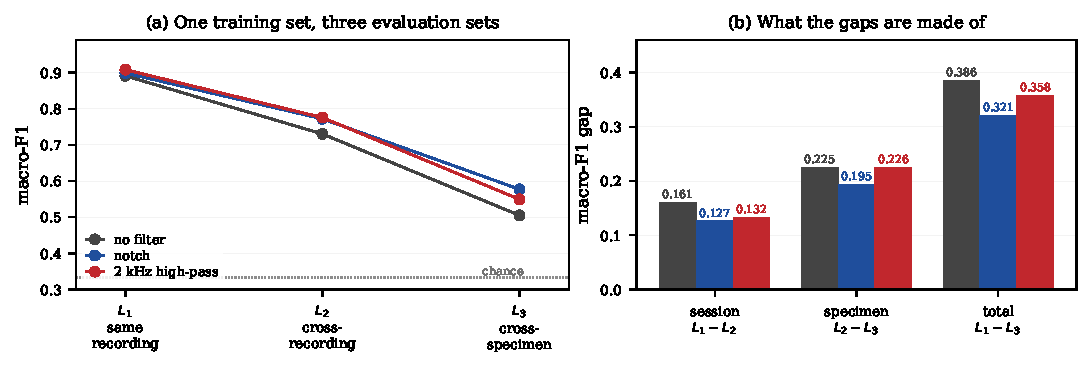
\includegraphics[width=0.98\textwidth]{figs/fig_pb_levels.pdf}
\caption{The decomposition of Table~\ref{tab:pb_levels}, and the same
decomposition with the rig tone removed. (a)~One training set, three
evaluation sets that differ by one factor each; the drop between consecutive
markers is exactly one of the terms plotted in (b). The three curves are the
unfiltered data and the two filtered variants: removing $93.3\%$ (notch) or
$99.7\%$ (high-pass) of the spectral energy moves any level by at most $0.07$
and does not remove the decline.
(b)~The two terms and their sum, bars are means over ten seeds. Filtering
reduces the session term from $0.161$ to $0.127$ and $0.132$, roughly a fifth,
and leaves the specimen term without a consistent direction ($0.225$ to $0.195$
and $0.226$), so the total stays in $0.32$--$0.36$.}
\label{fig:pb_levels}
\end{figure*}

\subsection{Where the kinematics match the labels}

The Paderborn classes are defined by damage location, so here the impulse train
at BPFO/BPFI is the right physics for the label. We therefore repeat the
no-source few-shot experiment of Section~\ref{sec:results} with these classes,
evaluating on held-out bearings.

\begin{table}[t]
\centering
\caption{No-source few-shot augmentation on Paderborn, classes defined by damage
location (healthy / inner ring / outer ring), bearing-disjoint test, macro-F1.
Chance is $0.333$. Five seeds at $k=5$, three at $k=20$ and $k=50$. The last
column is the same setting as
Table~\ref{tab:fewshot} except that the class labels are, on this benchmark,
consistent with the fault kinematics.}
\label{tab:pb_fewshot}
\small
\resizebox{\columnwidth}{!}{%
\begin{tabular}{lcccc}
\toprule
$k$ (windows/class) & Real support & Pure twin & Fingerprint & $+$ physics \\
\midrule
$5$  & $0.286$ & $0.166$ & $0.203$ & $0.199$ \\
$20$ & $0.316$ & $0.172$ & $0.177$ & $0.266$ \\
$50$ & $0.325$ & $0.166$ & $0.168$ & $0.231$ \\
\bottomrule
\end{tabular}
}
\end{table}

Three things are true in every row. Nothing beats simply training on the real
labeled samples. The pure twin is the \emph{worst} entry, below the chance level
of $0.333$, even though its physics matches the class definition exactly. And the
real-sample baseline does not improve with $k$ --- $0.286$ at five samples per
class, $0.325$ at fifty --- so the ceiling here is set by the bearing-disjoint
protocol, not by sample count. Within the augmentation columns the ordering is
stable too: layering the impulse train onto the target envelope is the highest
augmentation at $k=20$ ($0.266$ against $0.177$) and at $k=50$ ($0.231$ against
$0.168$), and is level with the envelope alone at $k=5$ ($0.199$ against
$0.203$). Both of those exceed the pure twin in all three rows.

The table cannot rank methods: every entry is at or below chance, and the
differences between the augmentation columns lie within one standard deviation.
We report it for the one comparison that is stable across all three values of
$k$, and that is externally corroborated.

\paragraph{A positive control for the mechanism}
On CWRU, fingerprint calibration was the best augmentation and layering physics
on it consistently hurt. On Paderborn the ranking inverts: fingerprint
calibration alone is indistinguishable from the raw twin, and adding the
physical impulse train is what recovers the ground it lost. This is exactly
what the mechanism predicts. On CWRU the class information \emph{is} the
fingerprint, so estimating the fingerprint captures the label and physics is
redundant noise. On Paderborn we measured that the class-mean fingerprints are
identical across classes (margin $+0.003$, Table~\ref{tab:bench}); calibrating
to them therefore transfers no label information, and the only thing left
carrying the label is the impulse repetition rate --- the physics. The failure
we diagnose therefore lies in applying physics-based augmentation to a benchmark
whose class labels are bound to individual recordings.

\section{Method: Target-Domain Spectral Envelope Calibration}
\label{sec:method}

Let $\{(\mathbf{x}_i,y_i)\}_{i=1}^{kC}$ be the labeled target support set for
$C$ classes. For class $c$ we estimate the magnitude envelope
\begin{equation}
A_c(f) \;=\; \frac{1}{|\mathcal{S}_c|}\sum_{i \in \mathcal{S}_c}
\bigl|\mathcal{F}\{ \mathbf{x}_i \odot \mathbf{w} \}(f)\bigr|,
\end{equation}
smoothed with a moving average of width $5$ bins and normalized to unit $\ell_2$
norm. Every envelope number quoted in this paper (hereafter the \emph{smoothed
envelope}) uses this definition; the unsmoothed class-mean spectra of
Table~\ref{tab:bench} are a different statistic and are not comparable to it.
Synthetic samples are then obtained by coloring an excitation $e$ in the
frequency domain,
\begin{equation}
\mathbf{x}_{\text{syn}} = \mathcal{F}^{-1}\bigl\{\, \mathcal{F}\{e\} \cdot A_c \,\bigr\},
\end{equation}
followed by per-window $z$-scoring. We consider two excitations: white noise
(the \emph{fingerprint} variant) and an impulse train placed at the
characteristic frequencies recomputed at the \emph{target} shaft speed
(the \emph{fingerprint$+$physics} variant).

Both variants use only the $k$ labeled support samples; no test window is
involved. The envelopes are accurate at small $k$: estimated from $k=5$
samples, the per-class envelope matches one estimated from the entire target
load at cosine $0.995$ on average ($0.989$ worst class). The corresponding
\emph{source-domain} envelopes match the target load only at $0.924$, which is
why the target-domain qualifier matters.

\section{Results}
\label{sec:results}

\subsection{Standard protocol}
Table~\ref{tab:main} reports the ten-class S0$\rightarrow$S3 comparison,
five seeds, all runs from a single uniform batch. Three observations.

\emph{The twin is worse than its own ablation.} Adding the calibrated physics
twin (\ml{dt\_dann}) reaches macro-F1 $0.914 \pm 0.078$, below plain adversarial
adaptation (\ml{dann}, $0.986 \pm 0.027$) and below the physics-free
augmentation ablation \ml{rand\_dann} ($0.922 \pm 0.098$). It is also the least
stable configuration.

\emph{The protocol saturates.} Every configuration that uses target labels
reaches $0.91$--$1.00$, leaving almost no headroom; the differences among
\ml{dann}, \ml{fp\_phys\_dann} and \ml{fp\_dann} are not a meaningful
demonstration of method quality in this regime. The informative comparisons are
in the constrained regimes of Section~\ref{sec:constrained}.

\emph{Performance is bounded by the labeled support set.} The zero-label bound
\ml{src\_pure} reaches $0.731$; merely adding the $k=5$ labeled target samples
(\ml{source\_only}) raises this to $0.823$.

\begin{table}[t]
\centering
\caption{Ten-class CWRU S0$\rightarrow$S3, $k=5$ labeled target samples per
class, five seeds, single uniform batch. \ml{src\_pure} uses no target data at
all; \ml{source\_only} and all remaining rows additionally use the labeled
support set.}
\label{tab:main}
\small
\resizebox{\columnwidth}{!}{%
\begin{tabular}{lcc}
\toprule
Method & Accuracy & macro-F1 \\
\midrule
\ml{src\_pure} (no target data)   & $0.8188 \pm 0.0421$ & $0.7307 \pm 0.0225$ \\
\ml{source\_only}                 & $0.8842 \pm 0.0377$ & $0.8228 \pm 0.0686$ \\
\ml{dann} (A2 ablation)           & $0.9904 \pm 0.0179$ & $0.9858 \pm 0.0268$ \\
\ml{rand\_dann} (A3 ablation)     & $0.9512 \pm 0.0553$ & $0.9223 \pm 0.0977$ \\
\ml{dt\_dann} (physics twin)      & $0.9028 \pm 0.1212$ & $0.9141 \pm 0.0780$ \\
\ml{fp\_phys\_dann} (fp.\ $+$ imp.)& $0.9917 \pm 0.0091$ & $0.9891 \pm 0.0123$ \\
\textbf{\ml{fp\_dann} (fp.\ $+$ noise)} & $\mathbf{0.9998 \pm 0.0003}$ & $\mathbf{0.9998 \pm 0.0004}$ \\
\bottomrule
\end{tabular}
}
\end{table}

\subsection{Constrained regimes}
\label{sec:constrained}
The standard protocol saturates, so the meaningful comparisons are the
constrained ones. In the synthesis-only regime (Table~\ref{tab:synth}) the
physics twin is at chance ($0.123$) while fingerprint-coloured white noise
reaches $0.910$; adding the physical impulse train drops this to $0.651$, and
removing the fault-harmonic fine structure from the envelope drops it further
to $0.524$.

In the no-source regime, where only the $k$ labeled target samples are
available (Table~\ref{tab:fewshot}), the same ordering holds: the twin
augmentation is harmful at every $k$, whereas spectral augmentation
helps, and most at $k=1$ ($0.890 \rightarrow 0.977$). Source-domain
fingerprints, which need no target labels, remain clearly worse than
target-domain ones at every $k$ ($0.861$/$0.905$ against $0.977$/$0.993$).

\begin{table}[t]
\centering
\caption{No-source few-shot setting, target load~3, macro-F1. Each cell is $6$
runs (three seeds, the whole configuration repeated twice).
Augmentations add $400$ samples per class generated from the $k$ labeled
support samples only.}
\label{tab:fewshot}
\small
\begin{tabular}{lccc}
\toprule
Augmentation & $k=1$ & $k=3$ & $k=5$ \\
\midrule
none (support only)        & $0.890$ & $0.970$ & $0.985$ \\
physics twin               & $0.558$ & $0.777$ & $0.885$ \\
fingerprint $+$ white noise& $0.977$ & $0.995$ & $0.993$ \\
fingerprint $+$ impulse     & $0.947$ & $0.983$ & $0.658^{\dagger}$ \\
source fingerprint         & $0.861$ & $0.945$ & $0.905$ \\
phase surrogate            & $0.960$ & $0.993$ & $0.993$ \\
noise-only augmentation    & $0.952$ & $0.991$ & $0.994$ \\
true target samples (bound)& $1.000$ & $1.000$ & $1.000$ \\
\bottomrule
\end{tabular}
\\[2pt]
\footnotesize $^{\dagger}$ very high variance ($\pm 0.46$): two of six runs
collapse to $0.014$, well below the $0.10$ chance level. The sample is bimodal
rather than noisy.
\end{table}

\section{Discussion and Limitations}
\label{sec:discussion}

\paragraph{Scope} The conclusion concerns the benchmarks rather than
simulation-based augmentation in general: the two datasets we examine cannot
test it, for different reasons that share a root.
On CWRU the class label is confounded with the recording, so the signal a
classifier learns is not the fault. On Paderborn the label \emph{is} physically
meaningful --- damage location, the very quantity whose characteristic
frequencies a model can compute --- yet the magnitude spectrum carries none of
it, because a single rig tone and its spectral leakage hold over $99\%$ of the
energy in every bearing whether healthy or damaged. A benchmark suitable for testing
physics-based augmentation must satisfy both conditions at once: the label must
have a physical definition, and the recording must actually expose it. Neither
of the two most-used public datasets does, and we suggest that establishing this
be part of benchmark validation rather than something each paper discovers
separately. The CWRU benchmark has already been criticised on related grounds
\cite{hendriks2022benchmark}; we add a mechanism and a quantitative control.
The situation is not unique to this field --- a model can generalise across
hospitals while relying on a site-specific confounder invisible in the
acquisition protocol \cite{zech2018variable} --- which is why we state the
requirement in terms of benchmark construction rather than of any one paper's
methodology.

This also reframes what the field should take from negative results. The
failure we diagnose is a property of the \emph{pairing} of a generator with a
benchmark, not of the generator. The same twin that is worthless on CWRU is, on
Paderborn, no longer the worst entry once its impulse train is layered onto the
target spectral envelope (Table~\ref{tab:pb_fewshot}): that is the only setting
in which we observe the physical component adding anything, and it is what the
mechanism predicts, since there the fingerprint carries no label and the only
remaining carrier of the label is the impulse repetition rate. The pure twin
remains the worst augmentation on \emph{both} benchmarks, and on neither does
any augmentation reliably beat training on the real labeled support samples.

\paragraph{Implications for reported numbers} Two papers reporting the same
method on CWRU may differ by $0.1$--$0.3$ macro-F1 purely because of how the
few-shot split was drawn. Future work should state whether support and test
come from the same recording, and ideally report both. The same control is
cheap wherever a dataset contains several independent specimens per class: hold
out specimens, not windows. Our own experience is a case in point. The
secondary tables in this paper are reported over six, ten or twenty runs rather
than the conventional three, because repeated execution of \emph{the same command}
with the same seeds moved a ten-seed mean by up to $0.033$ and made a
three-seed standard deviation wrong by more than an order of magnitude. This is
the same problem that has been documented for reinforcement learning
\cite{henderson2018matters} and for evaluation budgets generally
\cite{dodge2019showyourwork}, and it argues for reporting score
\emph{distributions} and the compute spent on them.

\paragraph{A benchmark validity checklist} The failures above share a
structure: a benchmark can make a positive or a negative result about
simulation-derived samples uninterpretable before any method is run.
Table~\ref{tab:checklist} states the properties a benchmark must have, the check
that establishes each, the signature of its failure, and where this paper
observes that signature. The first two rows cost nothing beyond a second
evaluation, the third is one FFT per class, and we suggest reporting all three
in the paper rather than in a supplement. The fourth row is a different matter:
Section~\ref{sec:pb_filter} shows that filtering the dominant line out of the
data does not remove the leakage, so observability and leakage have to be
checked separately rather than one standing in for the other.

\begin{table*}[t]
\centering
\caption{A benchmark validity checklist for simulation-based augmentation. Each
row is a property a benchmark must have before a positive or a negative result
about simulation-derived samples can be interpreted; the last column records
where this paper observes the corresponding failure.}
\label{tab:checklist}
\footnotesize
\begin{tabular}{@{}>{\raggedright\arraybackslash}p{0.15\linewidth}>{\raggedright\arraybackslash}p{0.34\linewidth}>{\raggedright\arraybackslash}p{0.25\linewidth}>{\raggedright\arraybackslash}p{0.18\linewidth}@{}}
\toprule
Dimension & Required check & Signature of failure & Observed here \\
\midrule
Specimen independence & Each class contains independent bearings, and no
specimen contributes to both support and test & One bearing reused across the
split & CWRU: one bearing per class \\
Recording independence & Support and test from different recordings; report both
numbers and the support-only baseline & A random window split of one recording,
so that using any target label beats training on the support set & CWRU:
$+0.15$--$0.19$ \\
Spectral separability & Within- versus between-class mean spectra, in source and
target & Between-class separation no larger than within-class & Paderborn:
margin $+0.003$ \\
Physical observability & Fault characteristic frequencies visible above the
recording's own structure & A rig tone or recording fingerprint dominates the
band & Paderborn: $100$\,Hz line, over $99\%$ of the energy \\
Temporal scale & The window spans several characteristic periods at the
sampling rate & The window holds about one fault cycle & Paderborn: $1024$
samples $=16$\,ms, one BPFO period \\
Synthetic validity & Synthetic and real class-conditional spectra agree, and a
discriminator cannot separate them & The generator reproduces no target class &
CWRU: twin macro-F1 $0.123$ \\
\bottomrule
\end{tabular}
\end{table*}

\paragraph{Limitations} (i) We study two datasets and two networks of the same
family, a full and a quarter-size ResNet; other architectures may behave
differently. (ii) The
cross-recording control on CWRU evaluates on a whole different load, which
confounds the recording change with the operating-condition change; a same-load,
different-session split is not available in CWRU, and we resort to Paderborn to
separate the two terms of Section~\ref{sec:paderborn}. There the separation
relies on $20$ repeated measurements per bearing, so it measures the session
term under one rig's repeat-measurement protocol and may not transfer to
datasets whose repeated recordings differ by more than a re-mount. (iii) Our
constructive method
is a regularizer rather than a uniform improvement, and we report it as such.
(iv) In the Paderborn subset we downloaded, every artificial-damage bearing is
outer-ring and every run-to-failure bearing is inner-ring, so damage location
and damage origin are confounded; our spectral claim is an \emph{absence} of
class structure and is unaffected, but it does not support a separate statement
about outer versus inner race. (v) The Paderborn few-shot entries all lie at or
below chance, so that table ranks nothing; we use it only for the two
comparisons that are stable across all three sample budgets. (vi) The spectral
comparison for Paderborn uses one operating condition and 21 bearings.

\section{Conclusion}
\label{sec:conclusion}

We showed that on CWRU cross-load bearing diagnosis the dominant class
information is a per-bearing recording fingerprint that physics cannot predict,
making simulation-based sample supplementation structurally ineffective on
that benchmark; that the standard few-shot protocol leaks this fingerprint from
support to test and inflates reported macro-F1 by $0.15$--$0.19$, rising to
$0.31$ in the hardest direction; and that a compact spectral envelope
calibration estimated from five labeled samples per class is the most robust
augmentation available, while adding physical impulse structure on top of it
consistently hurts.

A second benchmark tests whether this picture is specific to CWRU. On
Paderborn, where several independent bearings share each class, class-mean
magnitude spectra of healthy, inner-ring and outer-ring bearings are
indistinguishable (margin $+0.003$ after the rig tone is filtered out, against
$0.626$ on CWRU), so CWRU's class separation is a property of individual
specimens rather than of the classes. Same-recording evaluation there is still
optimistic, by $+0.386$, of which $+0.161$ is attributable to the recording
session alone and $+0.225$ to the change of specimen. Removing the rig tone,
which holds $93\%$ of the spectral energy, leaves $+0.321$, still dominated by
the specimen term, so the optimism is not an artefact of that line. The
physical component of the twin becomes useful for the first time once its
impulse train is layered on the target envelope, the one setting where the
labels rather than the fingerprints carry the physics --- though the pure twin
is still the worst augmentation there, and under cross-recording or
bearing-disjoint evaluation no augmentation on either benchmark reliably beats
training on the real labeled support samples. The practical
recommendation is to validate the benchmark before trusting either the positive
or the negative result obtained on it.

\bibliographystyle{IEEEtran}
\bibliography{refs}

\end{document}
